\section{Задача 2.8}
\subsection{Задание:}
Доказать, что если в результате конечного числа рациональных операций (сложение, умножение, вычитание, деление)
выполненых над комплексными числами $ z_1, \dots, z_n $ получается комплексное число $ u $, то в результате выполнения тех же
операций над $ \overline{z_1}, \dots, \overline{z_n} $ получается $ \overline{u} $.
\subsection{Доказательство:}
Пусть $ u_j $ - результат выполнения данных операций с числами $ z_1, \dots, z_j $,
тогда $ u_j = u_{j-1} \; \circ \; z_j $.
\\
Получается что $ u_n = u, \; \overline{u_n} = \overline{u} $.
\\
Докажем что $ \overline{u_j} $ - результат выполнения данных операций с $ \overline{z_1}, \dots, \overline{z_j} $
для каждой из четырёх операций:
\subsection{Сложение:}
$
	\overline{u_j}
	=
	\operatorname{Re} \overline{u_j} + i \operatorname{Im} \overline{u_j}
	=
	\operatorname{Re} u_j - i \operatorname{Im} u_j
	=
	\operatorname{Re} u_{j-1} + \operatorname{Re} z_j - i(\operatorname{Im} u_(j-1) + \operatorname{Im} z_j)
	=
	(\operatorname{Re} u_{j-1} - i\operatorname{Im} u_{j-1}) + (\operatorname{Re} z_j - i\operatorname{Im} z_j)
	=
	\overline{u_{j-1}} + \overline{z_j}
$
\subsection{Вычитание:}
$
	\overline{u_j}
	=
	\operatorname{Re} \overline{u_j} + i \operatorname{Im} \overline{u_j}
	=
	\operatorname{Re} u_j - i \operatorname{Im} u_j
	=
	\operatorname{Re} u_{j-1} - \operatorname{Re} z_j - i(\operatorname{Im} u_(j-1) - \operatorname{Im} z_j)
	=
	(\operatorname{Re} u_{j-1} - i\operatorname{Im} u_{j-1}) - (\operatorname{Re} z_j - i\operatorname{Im} z_j)
	=
	\overline{u_{j-1}} - \overline{z_j}
$
\subsection{Умножение:}
$
	\overline{u_j}
	=
	\operatorname{Re} \overline{u_j} + i \operatorname{Im} \overline{u_j}
	=
	\operatorname{Re} u_j - i \operatorname{Im} u_j
	=
	\operatorname{Re} u_{j-1} \cdot \operatorname{Re} z_j - i(\operatorname{Im} u_{j-1} \cdot \operatorname{Im} z_j)
	=
	\operatorname{Re} u_{j-1} \cdot \operatorname{Re} z_j +
	i(\operatorname{Im} \overline{u_{j-1}} \cdot \operatorname{Im} \overline{z_j})
	=
	\overline{u_{j-1}} \cdot \overline{z_j}
$
\subsection{Деление:}
$
	\overline{u_j}
	=
	\operatorname{Re} \overline{u_j} + i \operatorname{Im} \overline{u_j}
	=
	\operatorname{Re} u_j - i \operatorname{Im} u_j
	=
	\overline{u_{j-1}} / \overline{z_j}
$
\\[2em]
Таким образом в результате тех же операций над $ \overline{z_1}, \dots, \overline{z_n} $ получается $ \overline{u} $.
\subsection{Компьютерная проверка в среде Wolfram Mathematica:}
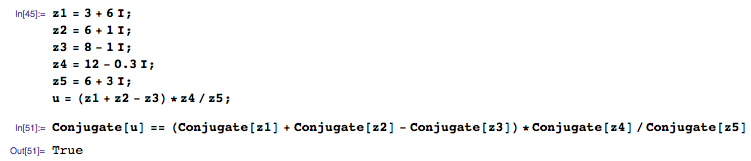
\includegraphics[scale=0.6]{task/2_08/screen1.png}
\\
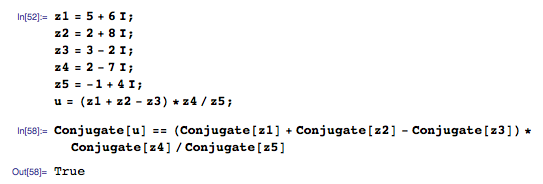
\includegraphics[scale=0.6]{task/2_08/screen2.png}
\subsection{Вывод:}
Утверждение доказано.
